\documentclass[journal]{IEEEtran}
\hyphenation{op-tical net-works semi-conduc-tor}
\setcounter{tocdepth}{2}


\usepackage{url}
\usepackage{cite}
%\usepackage[margin=1in]{geometry}
\usepackage[latin1]{inputenc}
\usepackage{graphicx}
\usepackage{listings}
\usepackage{color}
\usepackage{xcolor}
\usepackage{paralist}
\usepackage{caption}
\usepackage{subcaption}


\usepackage{hyperref}
\hypersetup{
    colorlinks,
    citecolor=black,
    filecolor=black,
    linkcolor=black,
    urlcolor=black
}

\usepackage{tikz}
\usepackage{tikz-er2}
\usetikzlibrary{shapes,arrows}
\usetikzlibrary{positioning}
\usetikzlibrary{shadows}
\tikzstyle{every entity} = [top color=white, bottom color=blue!30,
                            draw=blue!50!black!100, drop shadow]
\tikzstyle{every weak entity} = [drop shadow={shadow xshift=.7ex,
                                 shadow yshift=-.7ex}]
\tikzstyle{every attribute} = [top color=white, bottom color=yellow!20,
                               draw=yellow, node distance=1cm, drop shadow]
\tikzstyle{every relationship} = [top color=white, bottom color=red!20,
                                  draw=red!50!black!100, drop shadow]
\tikzstyle{every isa} = [top color=white, bottom color=green!20,
                         draw=green!50!black!100, drop shadow]
\tikzstyle{decision} = [diamond, draw, fill=blue!20,
    text width=4.5em, text badly centered, node distance=3cm, inner sep=0pt]
\tikzstyle{block} = [rectangle, draw, fill=blue!20,
    text width=5em, text centered, rounded corners, minimum height=4em]
\tikzstyle{edge} = [draw,line,-]
\tikzstyle{line} = [draw, -triangle 45]
\tikzstyle{cloud} = [draw, ellipse,fill=red!20, node distance=3cm,
    minimum height=2em]
\tikzstyle{dot} = [draw, circle, inner sep=1pt, fill=black]
\tikzstyle{db} = [draw,
  shape=cylinder,
  aspect=0.7,
  minimum height=2.5cm,
  minimum width=1.5cm,
  left color=yellow!30,
  right color=yellow!60,
  middle color=yellow!20, % Has to be called after left color and middle color
  outer sep=-0.5\pgflinewidth, % to make sure the ellipse does not draw over the lines
  shape border rotate=90
]


\definecolor{dkgreen}{rgb}{0,0.6,0}
\definecolor{gray}{rgb}{0.5,0.5,0.5}
\definecolor{mauve}{rgb}{0.58,0,0.82}
\lstset{ %
  language=SQL,                % the language of the code
  basicstyle=\footnotesize,           % the size of the fonts that are used for the code
  numbers=none,                   % where to put the line-numbers
  numberstyle=\tiny\color{gray},  % the style that is used for the line-numbers
  stepnumber=2,                   % the step between two line-numbers. If it's 1, each line 
                                  % will be numbered
  numbersep=5pt,                  % how far the line-numbers are from the code
  showspaces=false,               % show spaces adding particular underscores
  showstringspaces=false,         % underline spaces within strings
  showtabs=false,                 % show tabs within strings adding particular underscores
  rulecolor=\color{black},        % if not set, the frame-color may be changed on line-breaks within not-black text (e.g. comments (green here))
  tabsize=2,                      % sets default tabsize to 2 spaces
  breaklines=true,                % sets automatic line breaking
  breakatwhitespace=false,        % sets if automatic breaks should only happen at whitespace
                                  % also try caption instead of title
  keywordstyle=\color{blue},          % keyword style
  commentstyle=\color{dkgreen},       % comment style
  stringstyle=\color{mauve},         % string literal style
  escapeinside={\%*}{*)},            % if you want to add LaTeX within your code
  morekeywords={*,...}               % if you want to add more keywords to the set
}

\colorlet{punct}{red!60!black}
\definecolor{background}{HTML}{EEEEEE}
\definecolor{delim}{RGB}{20,105,176}
\colorlet{numb}{magenta!60!black}
\lstdefinelanguage{json}{
    basicstyle=\scriptsize\ttfamily,
    showstringspaces=false,
    breaklines=true,
    literate=
     *{0}{{{\color{numb}0}}}{1}
      {1}{{{\color{numb}1}}}{1}
      {2}{{{\color{numb}2}}}{1}
      {3}{{{\color{numb}3}}}{1}
      {4}{{{\color{numb}4}}}{1}
      {5}{{{\color{numb}5}}}{1}
      {6}{{{\color{numb}6}}}{1}
      {7}{{{\color{numb}7}}}{1}
      {8}{{{\color{numb}8}}}{1}
      {9}{{{\color{numb}9}}}{1}
      {:}{{{\color{punct}{:}}}}{1}
      {,}{{{\color{punct}{,}}}}{1}
      {\{}{{{\color{delim}{\{}}}}{1}
      {\}}{{{\color{delim}{\}}}}}{1}
      {[}{{{\color{delim}{[}}}}{1}
      {]}{{{\color{delim}{]}}}}{1},
}


\newcommand{\pad}{\vbox to 20pt{}}


%-------------------------------------------------------
\begin{document}
\title{Designing a Minimalist CRUD System\\ for Android Clients}
\author{Anthony Naddeo \\ Advisor: Sudarshan Chawathe}

\maketitle


\begin{abstract}
CRUD applications are those that enable users to create, read, update and delete data from some specified data set, often times in a relational database. The differences between CRUD applications lie primarily in the data that they manage, not in features or expectations. We present a model for representing the relationship between the standard CRUD operations and the data that is being managed. With this model, it is possible to write a single CRUD application that can be used to manage any set of data that uses a relational database. We define a protocol that enables arbitrary amounts and types of clients to perform CRUD operations on the same database. We also present a protocol for replicating database instances across arbitrary DBMSs. These ideas have been combined into one easily deployable system that can be used to create and maintain CRUD applications without writing client source code.
\end{abstract}

\begin{IEEEkeywords}
Android, CRUD, meta model, database replication
\end{IEEEkeywords}

\IEEEpeerreviewmaketitle
\tableofcontents

%--------------------------------------------------------
\section{Introduction} \label{sec:intro}
%--------------------------------------------------------

% give some background and describe what the project does / how it works

% mention CRUD
% mention everyone is writing the same application
% mention you shouldn't have to learn android

The term CRUD refers to the four basic operations on persistent storage: create, read, update and delete. Many CRUD focused applications implement their persistence layers using relational databases. Of these applications, many require multiple users to be able to perform CRUD operations on the same database\footnote{give an example} from arbitrary client types (Android, Web etc.). The data managed by CRUD applications varies greatly, but functionality and user interfaces are largely the same across instances. For this reason, there have been many frameworks that aid developers in creating their own CRUD applications, but most of them require the programmer to write code (i.e. PHP or Java) in order to generate entire applications that can be installed or placed on a web server; this quickly complicates an otherwise simple application. 

The use of a framework should be a categorically simpler experience than building a CRUD application from scratch. Currently, the framework that best meets this requirement is called Evolutility, by Olivier Giulieri. Evolutility is effective because the programmer only has to create XML configuration files that describe UI forms that are generated at run time. This approach results in a generic application that can be configured to display any type of data without needing to edit the source. That being said, the project has some shortcomings, particularly in its lack of native mobile application support (Android specifically) and its dependency on proprietary Microsoft technology (as opposed to open standards like Apache, PHP and MySQL). 

In this paper, we expand the generic CRUD application model described by Giulieri\footnote{cite} to enable arbitrary client types and support mobile clients by adding features like database replication for off line reading. This project was originally an inventory application designed for Networkmaine, the ISP for the public schools and libraries of Maine; they will be the recurring theme in the examples of this paper. 


%--------------------------------------------------------
\subsection{Motivating Examples} \label{sec:motivation}
%--------------------------------------------------------

In this section, we provide examples that illustrate the initial constraints this project had to operate under in order to be effective. 

%--------------------------------------------------------
\subsubsection{Mobile phones are often off line}  \label{sec:offline}

Libraries often cannot afford dedicated technical staff. When equipment breaks, an employee of Networkmaine is likely to be dispatched to the site to install a replacement. The equipment at libraries is commonly stored in the basements where little-to-no wifi or mobile signal can reach. If the staff member does not know which of the two router ports should provide the site with internet, then, regardless of signal, they should be able to use their mobile device to retrieve that information.



%--------------------------------------------------------
\subsubsection{Some users will only use browsers}  \label{sec:browser}

There are many network tools that are available exclusively through browsers at Networkmaine. Mobile applications will have to coexist in the same system as web and desktop based applications.


%--------------------------------------------------------
\subsubsection{The database schema is likely to change over time}  \label{sec:change}

Most of the technical employees at Networkmaine are network engineers; very few of them are even familiar with Android development. All application maintenance will ultimately fall on the shoulders of someone who would rather being doing something else. It is reasonable to assume that they might need to start tracking other device types, or additional dates at some point in time. Changes of this sort should not require recompilation of the application or any source code modification.


%--------------------------------------------------------
\subsubsection{Entirely separate applications will eventually be needed}  \label{sec:deployable}

It is also reasonable to assume that Networkmaine may have a need to track something entirely unrelated to networking devices (enrollment information perhaps). Additional instances of CRUD applications should be easy to configure and deploy.


%--------------------------------------------------------
\subsection{Overview}  \label{sec:overview}

% describe the structure of this project, what was used. The user should not be surprised by any of the following main sections after this section. He should expect a "Mirror method / Sync" section, "JSON ui form model" section, etc.

% explain server setup

% explain server side technologies

% explain android client setup
% explain android client dependencies 

% explain JSON stuff based on evolutility


We are interested in creating a generic CRUD system that shares a single database among arbitrary amounts (and types) of clients. In order to be effective, it must 
\begin{inparaenum}
\item be easier to use than creating a CRUD application,
\item allow off line reading on mobile clients,
\item have easily deployable instances for different databases and
\item never require source code modification for updates\footnote{Bugs in the source code will clearly require more traditional updates, but clients should adapt to the addition of tables or columns to the database.}.
\end{inparaenum}
In order to meet these requirements, we must have a way of replicating databases across arbitrary DBMS, isolate the parts of application instances that need to be customized (i.e. name and icon), and describe the UI enough for clients to display lists and forms that enable CRUD operations. Giulieri summarized his efforts well in his entry into the Code Generator 2008 Competition\cite{giulieri_minimalist_2011}
\begin{quotation}
``We argue that the key concept here is the representation of UI Metadata and that with a proper set of fundamental UI widgets, most CRUD applications can be effectively designed without hand coding.''
\end{quotation}
We use Giulieri's Evolutility\cite{giulieri_evolutility_????} project as a starting point. Evolutility consists of various .aspx pages and dlls that need to be copied to a web server, along with some SQL scripts that need to be run to create tables that store meta data. Once the initial configuration is done, an XML file can be created that specifies the relation between fields on forms and entities in the database. The XML file format is specified in his Code Generator 2008 Competition entry\cite{giulieri_minimalist_2011}. 

In our project, \texttt{Coexist}, we use entirely different technologies. One of the goals of our project is to be more accessible than Evolutility by using open and free (as in money) software when possible; consequently, Coexist uses a typical LAMP stack for the server, instead of ASP.NET and SQL Server.

We use JSON instead of XML for the model. The framework is designed in such a way that XML support can be added in the future, but JSON will be supported from the start. The same XML data can usually be represented with fewer bytes in JSON and can also be easier to hand edit. In addition, we already had experience with Google's Gson library and there were no significant reasons to prefer XML.

As mentioned, the server side code is written in PHP and is designed as an API. The API exposes four resources to clients, each one fulfilling a particular responsibility.

\begin{itemize}
\item \textbf{/api/sync}: Provides clients with the rows of the database that they are missing based on timestamp information.
\item \textbf{/api/schema}: Sends SQL to the client that creates the necessary tables on its local database. The DBMS type must be supplied in requests (i.e. SQLite).
\item \textbf{/api/crud}: Sends the JSON model to the client so that it can create UI forms.
\item \textbf{/api/create}: Creates or updates rows on the server. These rows are retrievable through calls to /api/sync.
\end{itemize}

An Android client implementation has also been provided. It uses the recommended Java based tools from Google, as well as the Android Support library and the ActionbarSherlock library\cite{wharton_actionbarsherlock_????} for backwards compatibility. At the moment, these dependencies are required in order to produce a viable client, though this may change as older versions of Android are aged out. Using third party libraries can be risky at times, but even Google seems to have made use of ActionbarSherlock in their own applications\cite{google_baseactivity.java_????}.

For the database replication we require a server side DBMS that supports triggers (MySQL, PostgreSQL, etc.). The replication utilizes timestamps to synchronize clients. Since one of our goals is full off line readability, Coexist is most suitable for smaller sized databases (the entire database will be replicated on the client's internal storage).


%--------------------------------------------------------
\subsection{Related Works} \label{sec:related}
% talk about what people are doing to solve this at the moment

Evolutility\cite{giulieri_evolutility_????} was by far the closest match to what we were trying to do, but before finding it there were several other projects that were encountered and rejected for various reasons. Android Crud Code Generator (ACCG)\cite{popovski_android-crud-code-generator_????} and Phreeze\cite{hinkle_phreeze_????} are representative of the kinds of projects that we were finding. The first is targeted at Android and the second is PHP, but both of them aim to make the CRUD experience simpler. Phreeze is a polished application, but it requires users to write code during the "development" process, which violated our requirements. ACCG took a different approach. It generates all of the Java code that would be needed when making a CRUD application. This is similar from a user perspective, but we ultimately want to have one code base that never has to be modified; not to mention, it is strictly local storage. OpenMobster's CRUD Tutorial\cite{openmobster_mobilizehibernate_????} introduced us to the Hibernate framework\cite{jboss_community_hibernate_????} for object relational mapping. This is a mature framework that enables transparent persistence of Java objects. This violates our goal of minimizing requirements, as well as requiring code to be written; non the less, it is an impressive and interesting framework. 


%--------------------------------------------------------
\subsection{Outline of Paper} \label{sec:outline}

% explain what each section does

The remainder of this paper is organized as follows. Section~\ref{sec:xml} reviews the XML based meta model presented by Giulieri and Section~\ref{sec:json} introduces the JSON version of it used by Coexist. Section~\ref{sec:db} describes the protocol used to enable database replication across arbitrary DBMSs. In Section~\ref{sec:api}, we take a closer look at the structure of the web server and API, and what interaction with clients will look like. Section~\ref{sec:deployment} examines the system as a whole from the end user's perspective. It will also detail the work involved with customizing an Coexist instance and deploying it. We conclude in Section~\ref{sec:conclusion}.

%--------------------------------------------------------
\section{XML Meta Model} \label{sec:xml}
%--------------------------------------------------------


A \textit{meta model} is a model of a meta data. Giulieri defined the meta data (in this context) as ``the meaningful information necessary to fully describe the UI and database mapping''. In this section, we analyze a representative sample of one of Evolutility's XML meta models and explain the perceived reasoning behind its design. Understanding this XML meta model will make the design of the JSON version in Section~\ref{sec:json} clearer. Figure~\ref{fig:xml} contains the XML meta model sample.

\begin{figure}[h!]
\centering
\begin{lstlisting}[language=XML]
<?xml version="1.0" encoding="UTF-8"?>
<form label="To Do"  
      xmlns="http://www.evolutility.com">
  <data entity="task" entities="tasks" 
        icon="m-todo.gif" dbtable="EVOL_ToDo" 
        dborder="PriorityID, duedate" />
  <panel label="Task" width="62" >
    <field type="text" label="Title" 
      dbcolumn="title"
      required="1" cssclass="fieldmain" 
      maxlength="255" width="100" 
      search="1" searchlist="1" searchadv="1" />
    <field type="date" label="Due Date" 
      dbcolumn="duedate" 
      maxlength="10" width="40" 
      search="1" searchlist="1" searchadv="1" />
  </panel>
</form> 
\end{lstlisting}
\caption{Sample Evolutility XML meta model}
\label{fig:xml}
\end{figure}

Looking at the XML model it is obvious that the structure is designed around the user interface. This is noteworthy because the typical approach to relational-database-backed applications is encumbered by the object-relational impedance mismatch. When representing data in an object oriented language, one must agree upon a mapping from the relational database. Technologies like the Java Persistence API have attempted to solve this problem by allowing programmers to implicitly specify an object mapping when creating objects in code\cite{oracle_java_????}, but the approach presented in this section effectively side steps the issue by mapping the database directly to UI forms, where an obvious mapping \textit{does} exist.

With this in mind, it becomes easier to understand the semantics of the model. The root element is a \texttt{form}, inside of which are \texttt{data} and \texttt{panel} nodes. This information represents the structure of a \textit{ui form}, or a section of a graphical user interface that is dedicated to user input (like any paper form you may have encountered). The \texttt{field} nodes are the nodes that model the actual data in the database. These are grouped under \texttt{panel}s to represent sections of the UI, implemented, perhaps, using tabs. Each \texttt{field} contains attributes that specify certain database related attributes. A full list of attributes can be found on the original Evolutility submission page\cite{giulieri_minimalist_2011}.

\begin{itemize}
\item \textbf{\texttt{dbcolumn}}: The name of the column that this field represents. The name of the table is given in the \texttt{data} node. Each form ultimately models a table in the database.
\item \textbf{\texttt{label}}: A string that will represent this field in the UI.
\item \textbf{\texttt{type}}: The type of this field. Field types are not analogous with database types.
\item \textbf{\texttt{maxlength}}: Some UI metadata to allow visual customization. 
\item \textbf{\texttt{width}}: Similar to maxlength.
\item \textbf{\texttt{search}}: Specifies whether or not this field should appear in a search form. This allows users to hide fields that get auto populated from triggers.
\end{itemize}

Using this model, Evolutility generates web UI forms at run time. This means that no code has to be written for the developer to configure and change the applications functionality and appearance. 

The distinction between form types and database types is a flexible concept that enables additional UI functionality without jeopardizing the mapping between the database and UI. 


\begin{figure}[h!]
\centering
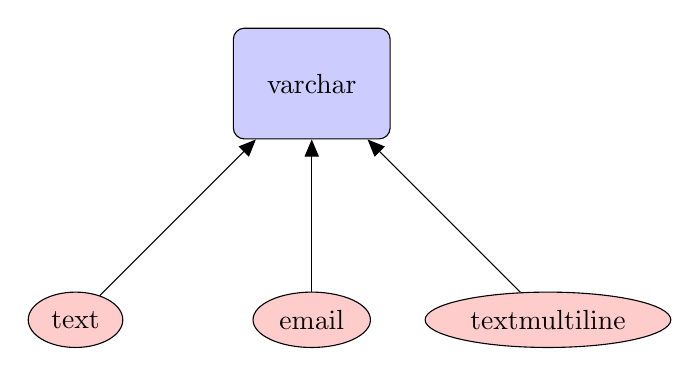
\begin{tikzpicture}[node distance = 2.5cm, auto]
  % Place nodes
  \node [block] (varchar) {varchar};
  \node [cloud, below of=varchar] (email) {email};
  \node [cloud, left of=email] (text) {text};
  \node [cloud, right of=email] (textm) {textmultiline};
  % Draw edges
  \path[line] (email) -- (varchar);
  \path[line] (text) -- (varchar);
  \path[line] (textm) -- (varchar);

\end{tikzpicture}
\caption{UI forms that map to the SQL \texttt{varchar} type.}
\label{fig:varchar_map}
\end{figure}

Figure~\ref{fig:varchar_map} shows the general relationship between UI types (shown in red) and SQL types (shown in blue). There are generally a number of UI types that map to a single database type. The difference between any two UI types that map to the same database type lie in their functionality. For example, the \texttt{text} UI type will cause fields to be presented as a single line of text, the \texttt{textmultiline} type will cause a fields to appear as text boxes, and the \texttt{email} type will cause fields to appear as a single line of text and enforce email style validation. 




%--------------------------------------------------------
\section{JSON Meta Model} \label{sec:json}
%--------------------------------------------------------

In this section, we examine the shortcomings of Evolutility and introduce a JSON model that is equivalent to the XML model of Section~\ref{sec:xml}. 



\begin{figure}[h!]
\begin{lstlisting}[language=json]
{
  "forms" : [
  {
    "label":"RMA",
    "table":"RMA",
    "fields": [
      {"label":"RMA Number","type":"barcode",
         "column":"rma_no"},
      {"label":"Sent","type":"date",
         "column":"sent"},
      {"label":"Returned","type":"text",
         "column":"returned"},
      {"label":"Note","type":"text",
         "column":"note"},
      {"label":"Serial","type":"reference",
       "column":"serial_no","required":true,
       "references":{
         "table":"Devices",
         "column":"serial_no"
    }}
    ]
  }
  ]
}
\end{lstlisting}
\caption{Sample JSON meta model.}
\label{fig:json_sample}
\end{figure}

The general form of the model is similar Evolutility's XML version. The first attribute in the object is \texttt{form}, which references an array of forms. Each form contains attributes that specify the database-UI mapping and UI metadata. The \texttt{label} and \texttt{table} of forms represent the title and the database table that it models, and the \texttt{fields} array contains \texttt{field} objects that model the actual data. The approach to \texttt{fields} has been altered and expanded. In the XML model, a foreign key was modeled as \texttt{lov} type (list of values). It would use integer primary keys to identify valid values in other tables. In Coexist, that type has been changed to the \texttt{reference} type, and an additional \texttt{references} attribute has been added to model the foreign key relationship, relieving the integer primary key requirement. In Figure~\ref{fig:json_sample}, the column \texttt{serial\_no} of table \texttt{RMA} is a foreign key on the \texttt{serial\_no} column in the \texttt{Devices} table. 

Since Coexist was designed with mobile clients in mind, there have been several UI types added to take advantage of smart phone functionality. The \texttt{barcode} type is the same as a \texttt{text} type, except it causes a barcode to appear on the right of it, allowing users to get input from a barcode using a smart phone's camera. The \texttt{image} type has been updated from Evolutility in this same fashion; it now presents a camera icon that allows users to receive input from a camera, ultimately mapping to a SQL \texttt{blob} type. The \texttt{location} data type allows users to use GPS as input, storing latitude and longitude information as a SQL \texttt{varchar} type\footnote{Many DBMSs provide types specifically for storing spatial data, but remaining DBMS independent and keeping restrictions low is currently prioritized higher.}. 






%--------------------------------------------------------
\section{The Server and API} \label{sec:api}
%--------------------------------------------------------

This section will explore some of the methods that the client can use to interface with the server, their advantages and disadvantages, and explain why the method labeled as the \textit{mirror method} is the appropriate choice. The following subsections will give details on the implementation of this method and its implications on the database schema; particularly, how normalized it should be and how to handle deletions. In all diagrams in this section, the arrows indicate the flow of data and the labels indicate the actions that cause them.

\subsection{Examining interface methods}

Many mobile applications are supplemented by a local database (typically SQLite). Some applications are stand alone and use these databases primarily as persistent storage; the Networkmaine inventory application uses its local database to interface with the remote back end MySQL server that it depends heavily on. There were three methods for this interfacing that represent different degrees of caching, from none, to selective, to complete.




%-------------------------------------------------------
\subsubsection{Window method}

In the window method, the data that a user sees at any given time is a window into the back end server; all of the data came from the server and none of it is going to persist beyond this screen. The major advantage to this method is its ease of implementation. This would be a suitable fit for a small weather application; in fact, it is the approach that my own weather application , QtWeather, uses.  

%TODO add some more analysis details

\begin{figure}[h!]
\centering
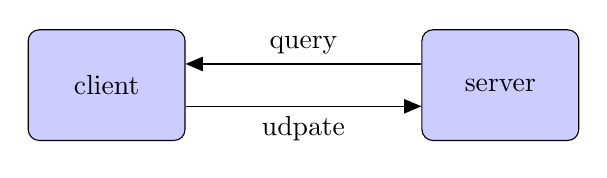
\begin{tikzpicture}[node distance = 2cm, auto]
  % Place nodes
  \node [block] (client) {client};
  \node [block, right of=client, node distance=5cm] (server) {server};
  % Draw edges
  \path [line] (server.165) -- node [above] {query} (client.15);
  \path [line] (client.345) -- node [below] {udpate} (server.195);
\end{tikzpicture}
\caption{Window method}
\label{fig:window}
\end{figure}


%-------------------------------------------------------
\subsubsection{Cache method}

Treating the client as a window requires that we don't have large amounts of data constantly being retrieved from the server. If this is not the case, then we may want to identify some data (or queries) that are commonly used in order to cache (and optionally sync) on the client's local database. This would be suitable for a mobile social networking client. Take a typical Facebook application for example; it would be advantageous to cache a users top five commonly used groups as well as their friend list because this information is supposedly accessed often and is relatively static. In contrast, caching the Facebook news feed would probably result in a lot of wasted space because of how fast it changes and how rarely old news feed entries are viewed. 



\begin{figure}[h!]
\centering
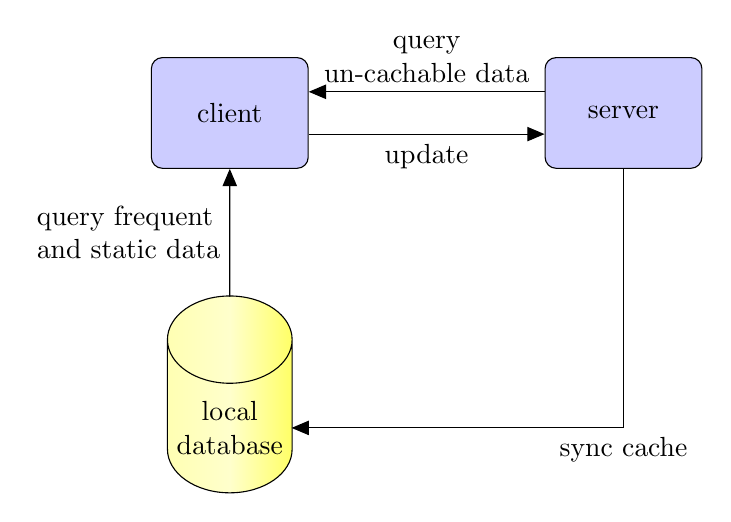
\begin{tikzpicture}[node distance = 2cm, auto]
  % Place nodes
  \node [block] (client) {client};
  \node [block, right of=client, node distance=5cm] (server) {server};
  \node [db, below of=client, node distance=4cm, align=center] (database) {local \\ database};

  % Draw edges
  % Need to align in order to line break
  \path [line] (server.165) -- node [above, align=center] {query \\ un-cachable data} (client.15);
  \path [line] (client.345) -- node [below] {update} (server.195);
  \path [line] (server) |- node {sync cache} (database);
  \path [line] (database) -- node [align=left] {query frequent \\ and static data} (client);
\end{tikzpicture}
\caption{Cache method}
\label{fig:cache}
\end{figure}


%-------------------------------------------------------
\subsubsection{Mirror method}
The window method has the client retrieve all data from the server all of the time, the cache method identifies some useful data to store and then caches it locally; the mirror method is the next natural step in this progression: cache the entire database. There are some immediate concerns with this approach, most prominent of which concerns the size of the database potentially being much larger than the what we can reasonably expect to store on the client. The advantages to this method are faster query times and less reliance on the network. In fact, this is the only method that would enable a fully readable database off line.

\begin{figure}[h!]
\centering
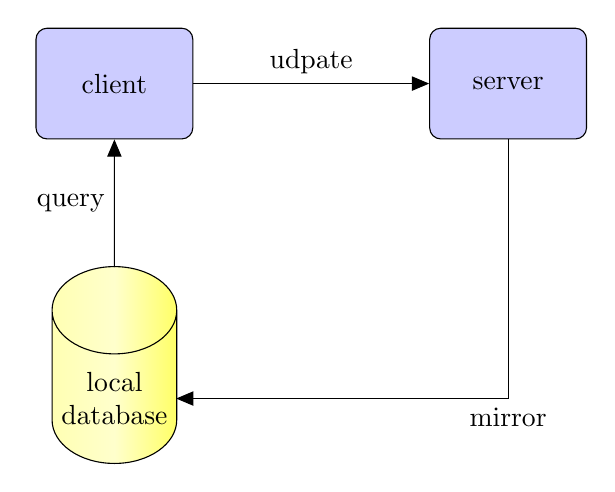
\begin{tikzpicture}[node distance = 2cm, auto]
  % Place nodes
  \node [block] (client) {client};
  \node [block, right of=client, node distance=5cm] (server) {server};
  \node [db, below of=client, node distance=4cm, align=center] (database) {local \\ database};

  % Draw edges
  % Need to align in order to line break
  \path [line] (client) -- node {udpate} (server);
  \path [line] (server) |- node {mirror} (database);
  \path [line] (database) -- node [align=left] {query} (client);
\end{tikzpicture}
\caption{Mirror method}
\label{fig:mirror}
\end{figure}

The Networkmaine inventory database contains information for approximately six thousand devices, location, purchase order and rma information for batches of devices; the size of the MySQL database dump is 1.5 megabytes. In addition, the database will not grow quickly. The size of the database makes the mirror method very attractive: if Networkmaine added two thousand units a year to its deployment then in twenty years the size of the database would be no less than 12 megabytes; still reasonable to store on the mobile clients we see available today (probably more so on the mobile clients in twenty years, if we still use them). Realistically, there won't be more than a few hundred devices added to the inventory each year, at most. It is for these reasons that the mirror method is preferable for this project. 


%-------------------------------------------------------
\subsection{Implementing the mirror method}

Many database systems support mirroring, or data replication. The driving factor in this technology seems to be data availability: always having a slave database server that can assume the primary role in the event that something goes wrong\cite{microsoft_database_????}. The issue here is that we don't have much control over the development environment; the server side database is MySQL because that is what the staff is familiar with and the client side database is SQLite because that is what Android supports. While MySQL does support data replication to MySQL slave servers, it certainly does not support replication to arbitrary alternative DBMS\cite{mySQL_mySQL_????}.

That does not mean it is impossible. We considered an interesting solution from fyreCloud's Amsler project. It was designed with Android in mind, attempting to mediate the MySQL replication protocol to make it compatible with SQLite\cite{fyrecloud_solutions_fyrecloud_????}. The actions of the Amsler project can be summarized as follows.

\begin{enumerate}
\item Configure the MySQL back end for data replication as described by the MySQL manual. 
\item Use TCP/IP connections to continuously push changes to the client in the form of MySQL commands.
\item Use a lexer and parser to map the incoming MySQL queries to valid SQLite queries. 
\end{enumerate}

Step 3 was troublesome; the syntax of different SQL implementations has many subtle differences. The idea of having a limited set of queries (dictated by the Amsler project's progress) that we could use on the server was too much to bear.

A simpler approach to this problem involved the addition of \textit{metacolumns} to the original schema; or columns defined in a SQL table that do not traditionally relate to the other columns in that table, but instead are used for some application level purpose. The most important of these metacolumns is the \texttt{mod\_ts} (modification timestamp) column. Let's take a simple relation \hbox{\texttt{Student(id, name, year)}} and examine how it can be synchronized across multiple instances without using any DBMS specific features. In this example, both the client and server tables are initialized to the table in Figure~\ref{fig:student_init}. 


\begin{figure}[h!]
\center
\begin{tabular}{ l | l | l || l }
id  & name      & year  & \textit{mod\_ts} \\
\hline  \hline
1   & Anthony   & 4     & \textit{0}        \\
2   & Lucas     & 3     & \textit{0}        \\
3   & Steven    & 3     & \textit{0}        \\
\end{tabular}
\caption{Initial state of the \texttt{Student} table.}
\label{fig:student_init}
\end{figure}

As implied, the \texttt{mod\_ts} metacolumn will be updated with the time of the transaction. For the purpose of readability, we represent this timestamp as the number of seconds since the creation of the table. 

Now lets update the server from one of the many possible client applications. 


\begin{figure}[h!]
\begin{lstlisting}
BEGIN TRANSACTION;
INSERT INTO Student(name,year) VALUES(Ryan, 4);
UPDATE Student SET year=4 WHERE name='Lucas';
COMMIT;
\end{lstlisting}
\caption{Transaction on the server.}
\label{fig:student_transaction1}
\end{figure}

It is worth mentioning now that the following trigger must exist on the server database for \texttt{INSERT}, \texttt{UPDATE} and \texttt{REPLACE} (but not necessarily for \texttt{DELETE}, explained in section \ref{sec:schema}).


\begin{figure}[h!]
\begin{lstlisting}
CREATE TRIGGER mod_ts AFTER INSERT ON Student
  FOR EACH ROW SET mod_ts = NOW();
\end{lstlisting}
\caption{Trigger for modification timestamps.}
\label{fig:student_trigger}
\end{figure}

The transaction of figure~\ref{fig:student_transaction1} will leave the server in the following state.

\begin{figure}[h!]
\center
\begin{tabular}{ l | l | l || l }
id  & name      & year  & \textit{mod\_ts} \\
\hline  \hline
1   & Anthony   & 4     & \textit{0}        \\
2   & Lucas     & 4     & \textit{10}        \\
3   & Steven    & 3     & \textit{0}        \\
4   & Ryan      & 4     & \textit{10}        \\
\end{tabular}
\caption{Server state after transaction of figure \ref{fig:student_transaction1}.}
\label{fig:student_update}
\end{figure}

Currently all clients are still in the state of figure~\ref{fig:student_update} and need to be synchronized with the server; this is a multi-part process, central to which is the client side query in figure~\ref{fig:student_change}. 

\begin{figure}[h!]
\begin{lstlisting}
SELECT max(mod_ts) FROM Student;
\end{lstlisting}
\caption{Find the most recent local change.}
\label{fig:student_change}
\end{figure}

In our case (and in many cases), the client communicates with the server database through a RESTful API. One such function provided by this API is $getChanges(table,~ts)$, where $table$ is the name of a table and $ts$ is a timestamp. In our running example, all clients would have to send a call to $getChanges(~Student,~0)$, where $0$ was returned from the query of figure~\ref{fig:student_change}. The server will respond to the client by returning all rows of the Student table where $mod\_ts > 0$, enabling the client to insert or replace them locally. If the most recent change on the client side is the same as the most recent change on the server then they are in sync\footnote{Recall from figure~\ref{fig:mirror} that the client never modifies its local database, it only requests synchronization from the server.}.


%--------------------------------------------------------
\section{Database Replication} \label{sec:db}
%--------------------------------------------------------

It is important to ensure that the client can never update the server if the client is out of sync, and the client must always have a way of re-syncing itself.
This can be achieved with two simple API functions, \texttt{/api/sync} and \texttt{/api/schema}; where one function requests missing information and another requests schema information. This design accounts for the database schema being upgraded on the server, and clients attempting to make changes to the database server when out of sync. Figure~\ref{fig:protocol} depicts the network dialog between a client and server where the client attempts to sync itself when it is using and old version of the database. 




\begin{figure}[h!]
\centering
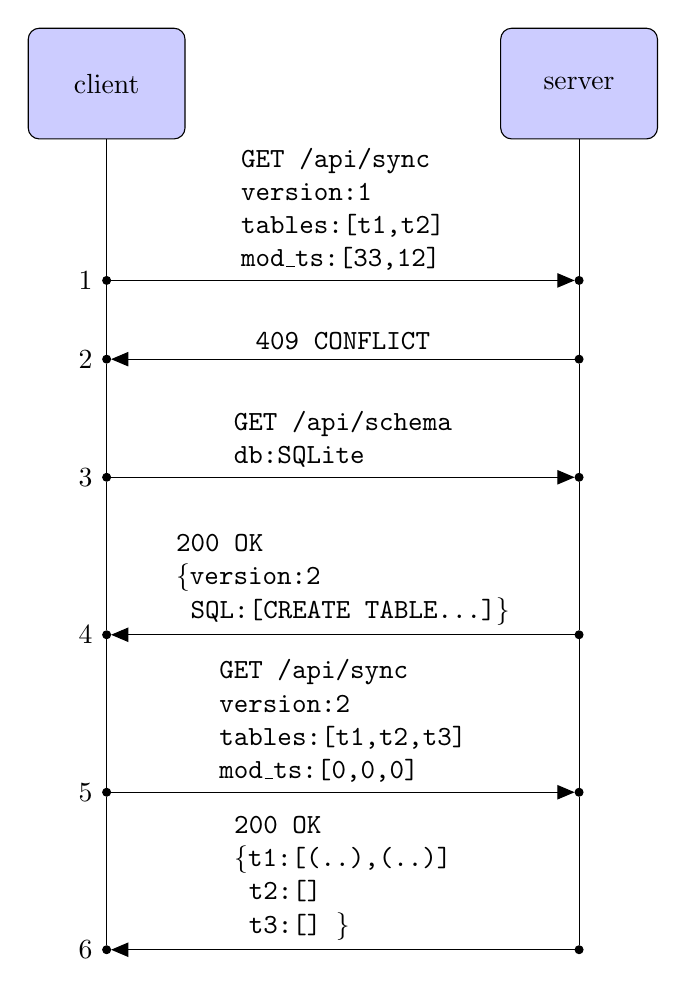
\begin{tikzpicture}[node distance = 2cm, auto]
  % Place nodes
  \node [block] (client) {client};
  \node [block, right of=client, node distance=6cm] (server) {server};
  
  \node [dot, below of=client, node distance=2.5cm, label=180:1] (c1) {};
  \node [dot, below of=server, node distance=2.5cm] (s1) {};
  \path [line] (c1) -- node [above, align=left] {
    \tt\textbf{GET /api/sync} \\ 
    \tt version:1 \\ 
    \tt tables:[t1,t2] \\ 
    \tt mod\_ts:[33,12]}   (s1);
  \path [edge] (client) -- (c1);
  \path [edge] (server) -- (s1);

  \node [dot, below of=c1, node distance=1cm, label=180:2] (c2) {};
  \node [dot, below of=s1, node distance=1cm] (s2) {};
  \path [line] (s2) -- node [above] {\tt\textbf{409 CONFLICT}} (c2);
  \path [edge] (c2) -- (c1);
  \path [edge] (s2) -- (s1);

  \node [dot, below of=c2, node distance=1.5cm, label=180:3] (c3) {};
  \node [dot, below of=s2, node distance=1.5cm] (s3) {};
  \path [line] (c3) -- node [above, align=left] {
    \tt\textbf{GET /api/schema} \\ 
    \tt db:SQLite            } (s3);
  \path [edge] (c2) -- (c3);
  \path [edge] (s2) -- (s3);

  \node [dot, below of=c3, node distance=2cm, label=180:4] (c4) {};
  \node [dot, below of=s3, node distance=2cm] (s4) {};
  \path [line] (s4) -- node [above, align=left] {
    \tt\textbf{200 OK} \\
    \tt\{version:2 \\
    \tt~SQL:[CREATE TABLE...]\} } (c4);
  \path [edge] (c3) -- (c4);
  \path [edge] (s3) -- (s4);
    
  \node [dot, below of=c4, node distance=2cm, label=180:5] (c5) {};
  \node [dot, below of=s4, node distance=2cm] (s5) {};
  \path [line] (c5) -- node [above, align=left] {
    \tt\textbf{GET /api/sync} \\ 
    \tt version:2 \\ 
    \tt tables:[t1,t2,t3] \\ 
    \tt mod\_ts:[0,0,0]}   (s5);

  \path [edge] (c5) -- (c4);
  \path [edge] (s4) -- (s5);


  \node [dot, below of=c5, node distance=2cm, label=180:6] (c6) {};
  \node [dot, below of=s5, node distance=2cm] (s6) {};
  \path [line] (s6) -- node [above, align=left] {
    \tt\textbf{200 OK} \\
    \tt \{t1:[(..),(..)] \\
    \tt~t2:[] \\
    \tt~t3:[] \}} (c6);
  \path [edge] (c6) -- (c5);
  \path [edge] (s6) -- (s5);

\end{tikzpicture}
\caption{Synchronization protocol}
\label{fig:protocol}
\end{figure}

The actions can be described as follows. 

\begin{enumerate}

\item The client sends a GET request to /api/sync on the server, including the database version it is using, an array of table names and an array of maximum modification timestamps for those tables (found in a metacolumn).

\item The server responds with a 409 error message because it is currently using version 2 of the database, while the client is using version 1.

\item The client sends a GET request to /api/schema on the server to get the current schema that the server side database is using. It requests the SQL in SQLite syntax.

\item The server responds with a 200 OK code. The body of the response is a JSON object containing the version of the server's database and the SQL statements that need to be executed in SQLite to build it. The constraints do not need to be sent to the client, only the table declarations (and possibly views). Since the client never updates its own database through SQL, the constraints are not necessary. 

\item The client now has enough information to re-create its database. Since there is nothing on the client that isn't also on the server, the client can simply replace the contents of its database with this new schema. A call to /api/sync is repeated with the new schema. 

\item There is no version conflict; the server responds with a 200 OK code. The body of the response is a JSON object that maps table names to arrays containing all of the tuples that the client is missing. 

\end{enumerate}


The dialog would look slightly different for an out of sync client attempting to make server changes. In figure~\ref{fig:protocol}, the client supplies the server with all of the tables and their most recent update timestamps. If the client was to send this information with each API request then the server could similarly notify the client when they appear out of date; but timestamps and table names can be verbose, it would better to send a representative checksum in their place. Figure~\ref{fig:signature} represents the sha1 checksum that can be sent in API requests as a \textit{signature} to validate the client; $T$ represents the concatenation of all table names, and $M$ represents the concatenation of all maximum modification timestamps. The first timestamp should correspond to the first table, and so on.

\begin{figure}[h!]
\[
sha1(version + T + M + username + sha1(password))
\]
\caption{API request signature.}
\label{fig:signature}
\end{figure}

So for a schema that consisted of the tables $Students$ and $Courses$, with maximum modification timestamps\footnote{These timestamps are the same ones depicted in figure~\ref{fig:student_init}} of $2012-12-01 16:18:31$ and $2012-12-01 16:18:43$ respectively, under version $1$ of the database, with a user name of $anthonyn$ and a password of $password$, the signature would be equal to \hbox{$9d64e5fbba865b491adeeeead91666df8d7cb1ec$}.

%begin{figure}[h!]
%sha1("1StudentsCourses2012-12-01 16:\\
%8:312012-12-01 16:18:43anthonyn5baa6\\
%e4c9b93f3f0682250b6cf8331b7ee68fd8") \\
% 9d64e5fbba865b491adeeeead91666df8d7cb1ec$
%caption{My Listing}
%label{fig:list}
%end{figure}

The popular client authentication method today is the OAuth library\cite{_oauth_????} used by Facebook, Twitter and LinkedIn to name a few. The idea is to use authentication tokens in place of passwords so that third party applications can access someone's information by making requests with tokens instead of passwords. For the purposes of Networkmaine, there will be no third party plug in service and all users access the same information over SSL. Storing local password hashes or requesting passwords per transaction (depending on user preferences) will suffice.







%-------------------------------------------------------
\subsection{Schema implications}
\label{sec:schema}

The synchronization depends on a few assumptions. If a row was deleted from the server then there would be no reliable way for the client to discover this using only the metacolumns. Assuming no insertions have taken place, missing rows would be $C - S$, where $C$ is the client side table and $S$ is the server side, but we would like to avoid sending the contents of entire tables over the network (aside from the initial synchronization). 

Many of the relations of our schema include timestamps to enable us to pose more interesting queries. For example, our \texttt{Shelved( serial\_no, date)} relation allows us to tell Networkmaine all of the devices that were shelved in a given time range; in the past, these devices might have been deleted from their records entirely. For this reason, and the reason in the prior paragraph, we decided it would be a good idea to never delete any data from the database. Instead, the \texttt{deleted} metacolumn was added to each relation; a simple boolean toggle that tells the application that this tuple should be considered deleted. This enables our synchronization method and preserves the integrity of queries that rely on having sufficient data to operate on.

Another practice to avoid is using relations to store states. In the original schema for Networkmaine, there was a table \hbox{\texttt{Shelved (serial, date, note)}} that was used to track devices that should be considered retired. These devices could potentially be used again and would have to be marked as deleted in the \texttt{Shelved} table with metacolumns. It is also reasonable to assume that the \texttt{Shelved} table's growth will mirror the \texttt{Device} table's growth because each new device will potentially replace an older device. 

One possible solution would be to merge the \texttt{Shelved} table into the \texttt{Device} table. In MySQL, a \texttt{BOOLEAN} occupies 1 byte, a \texttt{TIMESTAMP} occupies 4 bytes, and \texttt{VARCHAR} occupies at least 0 bytes and at most 3 bytes per character in utf-8 under the InnoDB engine. The initial database will have about six thousand devices in it, so merging the tables would add about $6000~bytes + 24000~bytes + 625~bytes \approx 30~kb$, or 5 bytes per row, where the $625~bytes$ came from the sum off all of the 1 bit bitmasks added for allowing \texttt{NULL} values in the \texttt{VARCHAR} column; a negligible amount for the small growth rate of the database. The updated table is shown in figure~\ref{fig:updated_device}.

 
\begin{figure}[h!]
\begin{lstlisting}
CREATE TABLE Device(
  serial VARCHAR(32) PRIMARY KEY,
  tag VARCHAR(32) NOT NULL,
  description VARCHAR(32),
  shelved BOOL DEFAULT FALSE NOT NULL,
  shelved_notes VARCHAR(32),
  shelved_date TIMESTAMP);
\end{lstlisting}
\caption{Updated \texttt{Device} table.}
\label{fig:updated_device}
\end{figure}



%--------------------------------------------------------
\section{Deployment} \label{sec:deployment}
%--------------------------------------------------------

% explain the application architecture 

% explain step by step.

In this section, we explain the process of deploying an instance of Coexist, using a shopping list application, ShoppingList, as an example. As the name implies, ShoppingList is an application that manages items on a shopping list. Since Coexist is designed to allow multiple clients edit a single set of data, it is a good fit for a household shopping list replacement. Before starting, you will need to have a few things.

\begin{enumerate}
\item Linux server with Apache and PHP5 installed. 
\item Eclipse or Ant
\end{enumerate}


%--------------------------------------------------------
\subsection{Create the database.}  \label{sec:}

ShoppingList is a simple application, consisting of one table called \texttt{Items}. Create the database and a user on the server, and execute the SQL to create the desired table and meta data trigger. Its not hard to manually create the triggers when there are few tables, but it can be tedious as more tables are added. In \texttt{web/bin}, there is a script called \texttt{mktriggers} that will parse SQL files and send triggers to stdout. A version of this file should also be saved in \texttt{web/lib/SQL/SQLite/1}. Saving it in this location means that it will be given to clients that use Sqlite for version \texttt{1} of the application.


\begin{figure}[h!]
\begin{lstlisting}
REATE TABLE Items(
  item VARCHAR(100),
  mod_ts DATETIME, --metacolumn
  deleted INTEGER, --metacolumn
  CONSTRAINT item_pk PRIMARY KEY (item)
);

CREATE TRIGGER Items_trigger 
  BEFORE UPDATE ON Items 
  FOR EACH ROW SET NEW.mod_ts=NOW();
\end{lstlisting}
\caption{ShoppingList SQL file.}
\label{fig:shoppinglist_SQL}
\end{figure}




%--------------------------------------------------------
\subsection{Create the JSON meta model.}  \label{sec:}

A simple database requires an equally simple JSON meta model. The following model will create a single \textit{Items} form on the client, consisting of the \texttt{text field} \textit{Item}. This file should be saved in \texttt{web/lib/ui/1/}, for the same reasons as the previous SQL file.

\begin{figure}[h!]
\begin{lstlisting}[language=json]
{
  "forms" : [
  { 
    "label":"Items",
    "table":"Items",
    "fields": [
    {"label":"Item", "type":"text","column":"item"}
    ]
  }
  ]
}
\end{lstlisting}
\caption{ShoppingList JSON meta model.}
\label{fig:shoppinglist_json}
\end{figure}


%--------------------------------------------------------
\subsection{Configure database credentials and version.}  \label{sec:}

In \texttt{web/conf} there is a file called \texttt{conf.ini} that provides PHP with some configuration info. Customize this as needed.

\begin{itemize}
\item \texttt{\textbf{version}}: The current version of the application. It is used to ensure that all clients are operating on the same database and UI. If this is incremented on the server then it will cause all clients to request SQL and JSON meta models for the new version.
\item \texttt{\textbf{user}}: The user name for the database for use by PHP.
\item \texttt{\textbf{pass}}: The password of the database user for PHP.
\item \texttt{\textbf{db}}: The name of the database. 
\item \texttt{\textbf{host}}: The host that the database resides on.
\item \texttt{\textbf{dbms}}: The DBMS (i.e. MySQL, PostgreSQL etc.)
\end{itemize}



%--------------------------------------------------------
\subsection{Deploy the PHP to the server.}  \label{sec:}

The server setup is flexible. In the web directory there is a script named \textit{deploy}. In that script there are two variables: \texttt{HOST} and \texttt{SRV}, where \texttt{HOST} is on the form \textit{user@hostname} and \texttt{SRV} is the path to the root web directory. So, if the server's IP address is 192.168.1.3, user is \texttt{anthony},and the web root is located at \texttt{/srv/shoppinglist.domain.org/htdocs}, then \texttt{HOST} is \texttt{anthony@192.168.1.3} and \texttt{SRV} is \texttt{/srv/shoppinglist.domain.org/htdocs}. Provided this information, the script will invoke \texttt{rsync} and copy the PHP code to the server. 



%--------------------------------------------------------
\subsection{Configure the Android application.}  \label{sec:}

The Android project has some things that need to be customized before installing. At the moment, the easiest way to do this is by opening up the project in an Android enabled Eclipse installation (the recommended Android development environment). Open the project in eclipse by importing it as an Android project. Right click the project in the explorer and select \texttt{Android -> Rename package}\footnote{This is particularly important if you plan on installing multiple instances of Coexist because identical package names will overwrite each other.}.For ShoppingList, it can be renamed to \texttt{org.domain.shoppinglist}. In \texttt{res/values/strings.xml}, change the \texttt{app\_name} to \texttt{ShoppingList}, and change \texttt{api\_baseurl} to \texttt{http://192.168.1.3/api}, since 192.168.1.3 is our server in this example.

There are also two different types of images used; \texttt{logo.png} is the icon for the application and \texttt{notification.png} is the icon for the notifications in the status bar.


%--------------------------------------------------------
\subsection{Build and install the Android application.}  \label{sec:}

In Eclipse, right click the project and select \texttt{Android -> Export application} to create an installable apk file. There are many ways of actually installing the application; use \texttt{adb} to transfer the apk to the device, host it on the web server and use the device's browser or mount the device in mass storage mode; whichever is easiest. Clicking on the apk will prompt an install.

%--------------------------------------------------------
\subsection{Start the Android application and let it sync.}  \label{sec:}

Once the application is installed and opened, the screen will be blank and spinning. 


\begin{figure}[h!]
\centering

\includegraphics[width=0.25\textwidth]{images/new.png}
\caption{ShoppingList on first launch.}
\label{fig:first_launch}
\end{figure}

In the overflow menu there is an option called \texttt{Sync Now} that will trigger a sync.


\begin{figure}[h!]
\centering
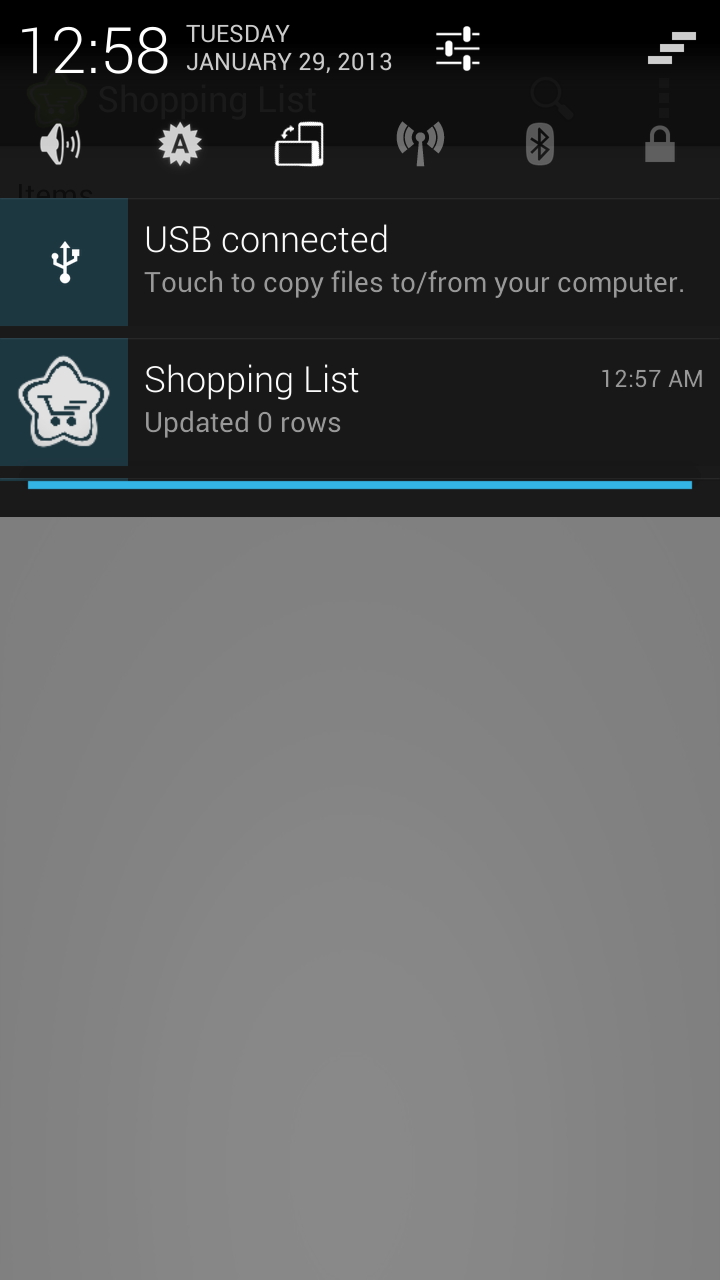
\includegraphics[width=0.25\textwidth]{images/dl.png}
\caption{ShoppingList after first sync.}
\label{fig:first_sync}
\end{figure}

This will cause the client to request the appropriate SQL file and JSON meta model file from the server. Using this, it will create a local version of the database and request all missing rows (which will be all rows). It will finish by reporting the total amount of rows that it received, as seen in Figure~\ref{fig:first_sync}


\begin{figure}[h!]
    \centering
    \begin{subfigure}[b]{0.1\textwidth}
        \centering
        
\includegraphics[width=\textwidth]{images/s1.png}
        \caption{Home}
        \label{fig:home}
    \end{subfigure}%
    ~ %add desired spacing between images, e. g. ~, \quad, \qquad etc.
      %(or a blank line to force the subfigure onto a new line)
    \begin{subfigure}[b]{0.1\textwidth}
        \centering
        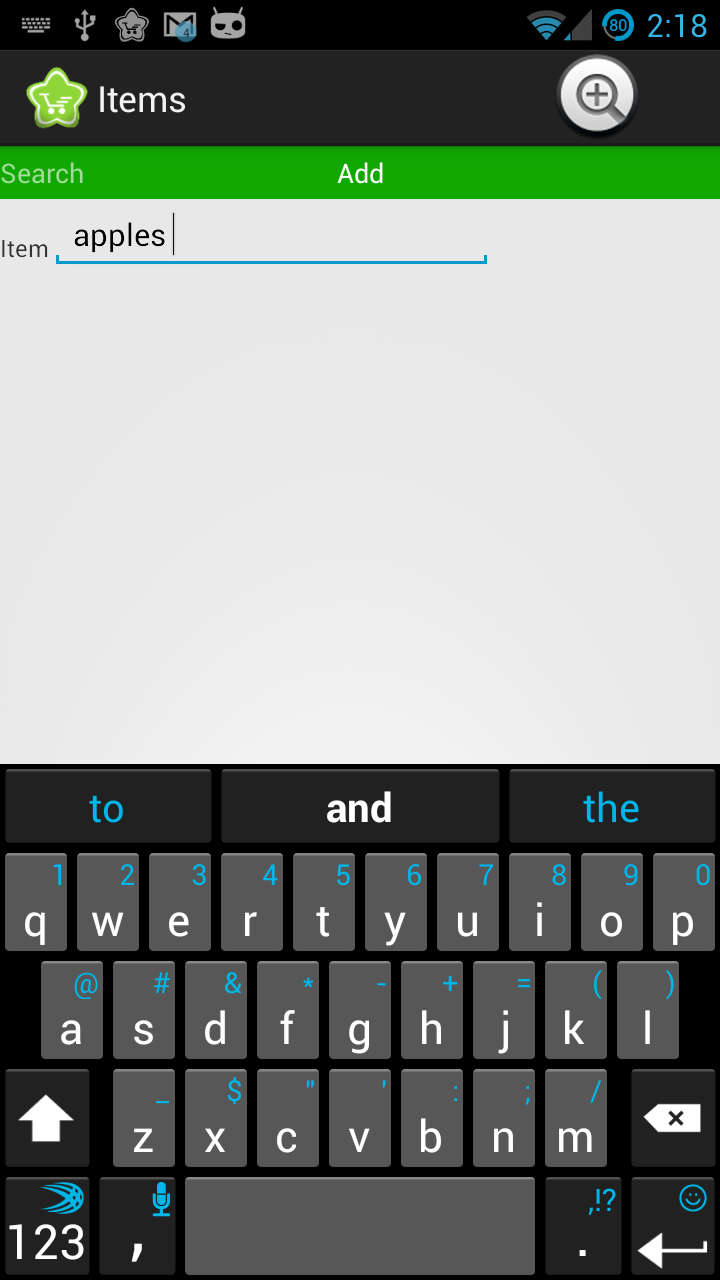
\includegraphics[width=\textwidth]{images/s2.png}
        \caption{Add}
        \label{fig:add}
    \end{subfigure}
    ~ %add desired spacing between images, e. g. ~, \quad, \qquad etc.
      %(or a blank line to force the subfigure onto a new line)
    \begin{subfigure}[b]{0.1\textwidth}
        \centering
        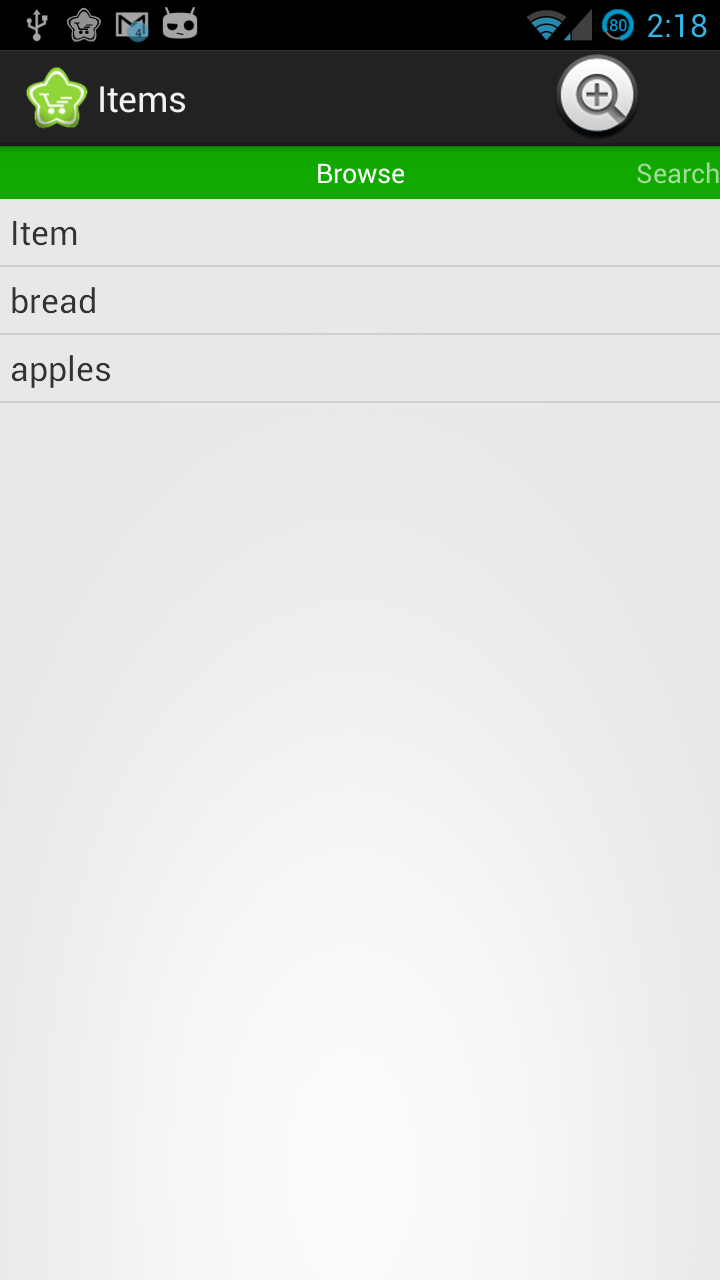
\includegraphics[width=\textwidth]{images/s3.png}
        \caption{Browse}
        \label{fig:browse}
    \end{subfigure}
    \caption{Final ShoppingList application screens.}\label{fig:shoppinglist}
\end{figure}


At this point the application is fully functional. Clicking on the \texttt{Items} section in the home screen will bring launch the CRUD screen for it. Swiping to the right will reveal the UI form generated by the JSON meta model and swiping to the left will allow browsing of the database contents. 

%--------------------------------------------------------
\section{Future Plans} \label{sec:}
%--------------------------------------------------------

Much of the setup work can be reduced to simple script execution. In the end, Coexist will be configurable through a dedicated tool that pulls down the latest stable code from whichever repository it is currently being hosted at and automatically configures it based on a name, domain, icon and server information.

%tools to auto generate JSON from SQL, or vice versa








%-------------------------------------------------------
% Bibliography
%-------------------------------------------------------
\bibliographystyle{IEEEtran}
\bibliography{report}
\end{document}


